% THIS IS SIGPROC-SP.TEX - VERSION 3.1
% WORKS WITH V3.2SP OF ACM_PROC_ARTICLE-SP.CLS
% APRIL 2009
%
% It is an example file showing how to use the 'acm_proc_article-sp.cls' V3.2SP
% LaTeX2e document class file for Conference Proceedings submissions.
% ----------------------------------------------------------------------------------------------------------------
% This .tex file (and associated .cls V3.2SP) *DOES NOT* produce:
%       1) The Permission Statement
%       2) The Conference (location) Info information
%       3) The Copyright Line with ACM data
%       4) Page numbering
% ---------------------------------------------------------------------------------------------------------------
% It is an example which *does* use the .bib file (from which the .bbl file
% is produced).
% REMEMBER HOWEVER: After having produced the .bbl file,
% and prior to final submission,
% you need to 'insert'  your .bbl file into your source .tex file so as to provide
% ONE 'self-contained' source file.
%
% Questions regarding SIGS should be sent to
% Adrienne Griscti ---> griscti@acm.org
%
% Questions/suggestions regarding the guidelines, .tex and .cls files, etc. to
% Gerald Murray ---> murray@hq.acm.org
%
% For tracking purposes - this is V3.1SP - APRIL 2009

\documentclass[]{sigcomm-alternate}
\usepackage{url}
%\usepackage[hidelinks]{hyperref}
\usepackage{multirow}
\usepackage[noend]{algpseudocode}
\usepackage{algorithm}
\usepackage{color}
\usepackage{verbatimbox}

\usepackage[pass]{geometry}
\setlength{\paperheight}{11in}
\setlength{\paperwidth}{8.5in}	

\newcommand{\ie}{i.e., \@}
\newcommand{\eg}{e.g., \@}
\newcommand{\Ie}{I.e., \@}
\newcommand{\Eg}{E.g., \@}

\renewcommand{\baselinestretch}{.990}

\newcommand{\todo}[1]{\textcolor{red}{TODO: \emph{#1}}}

\newcommand{\eat}[1]{}

\newenvironment{myitemize}
{
    \begin{list}{\labelitemi}{\leftmargin=1em}
        \setlength{\topsep}{0pt}
        \setlength{\parskip}{0pt}
        \setlength{\partopsep}{0pt}
        \setlength{\parsep}{0pt}         
        \setlength{\itemsep}{0pt} 
}
{
    \end{list} 
}

\begin{document}

\title{Awesome Project}
%\titlenote{(Does NOT produce the permission block, copyright information nor page numbering). For use with ACM\_PROC\_ARTICLE-SP.CLS. Supported by ACM.}
%\subtitle{[Extended Abstract]
%\titlenote{A full version of this paper is available as
%\textit{Author's Guide to Preparing ACM SIG Proceedings Using
%\LaTeX$2_\epsilon$\ and BibTeX} at
%\texttt{www.acm.org/eaddress.htm}}}
%
% You need the command \numberofauthors to handle the 'placement
% and alignment' of the authors beneath the title.
%
% For aesthetic reasons, we recommend 'three authors at a time'
% i.e. three 'name/affiliation blocks' be placed beneath the title.
%
% NOTE: You are NOT restricted in how many 'rows' of
% "name/affiliations" may appear. We just ask that you restrict
% the number of 'columns' to three.
%
% Because of the available 'opening page real-estate'
% we ask you to refrain from putting more than six authors
% (two rows with three columns) beneath the article title.
% More than six makes the first-page appear very cluttered indeed.
%
% Use the \alignauthor commands to handle the names
% and affiliations for an 'aesthetic maximum' of six authors.
% Add names, affiliations, addresses for
% the seventh etc. author(s) as the argument for the
% \additionalauthors command.
% These 'additional authors' will be output/set for you
% without further effort on your part as the last section in
% the body of your article BEFORE References or any Appendices.

\numberofauthors{1}
\author{
\begin{tabular}{@{\extracolsep{\fill}}ccc}
Dimitrios Sarlis & Federico Ponte & Gaurav Walia\\
\affaddr{Carnegie Mellon University} & \affaddr{Carnegie Mellon University} & \affaddr{Carnegie Mellon University}\\
\email{dimitris.sarlis@sv.cmu.edu} & \email{federico.ponte@sv.cmu.edu} & \email{gaurav.walia@sv.cmu.edu}
\end{tabular}\\
}

\maketitle


\begin{abstract}

Computing connected components of a graph is a well-known and thoroughly studied problem. It is also one of the fundamental subroutines in graph clustering or mining algorithms. Though there are a lot of algorithms that compute the connected components of a graph, many of them perform poorly when it comes to calculating the components in huge graphs such the ones that are created nowadays by social networks, web pages, etc. This leads us to other alternatives that can compute the connected components in a parallel way. In this project, we are particularly interested in Map-Reduce implementations of connected components to be able to scale our analysis to very large graphs with hundreds of millions of nodes and edges.

\end{abstract}



\section{Introduction}\label{sec:intro}
Very large scale graph mining is one of the most fundamental tools for modeling huge networks and is a very important problem in big data analytics nowadays. Examples of large graph datasets include webpages where the edges are the hyperlinks between documents and social networks that describe the relationships among people. In such networks, the problem of finding connected components is quite important as it is possible to extract useful information by grouping together connected vertices into sub-graphs.

First, we will introduce the problem of finding connected components in a graph formally. In graph theory, a connected component (or just component) of an undirected graph is a subgraph in which any two vertices are connected to each other by at least one path and they are not connected to other vertices in the supergraph. Figure \ref{figure:connected} shows the different connected components in a graph using a different color for each component.

\begin{figure}[!h]
 \centering
    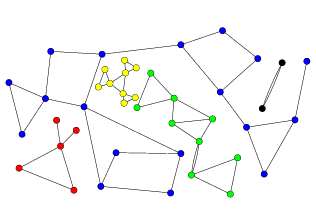
\includegraphics[height=12pc,width=15pc]{figures/connected_components.png}
	\caption{Connected components in a graph}
    \label{figure:connected}
\end{figure}

The problem of finding connected components is well-studied and there are a lot of previous works that have introduced a set of algorithms to address this problem in a MapReduce \cite{mapreduce} environment. Usually, these algorithms perform the computation in rounds of MapReduce jobs until some convergence criteria are met. These algorithms have various performance that depends on (i) total rounds of computation (in some cases it scales with the diameter of the graph), (ii) communication cost between two rounds of MapReduce and (iii) unbalanced workload on different machines that may slow down the total computation.

With the proliferation of social and information networks as well as with the huge amount of data contained in such networks, the problem of efficiently calculating connected components is not trivial. This makes the problem studied in the present work quite central in large-scale graph analysis. After computing the connected components in graphs, we can perform more complex graph analysis tasks, such as graph clustering which in the case of social graphs can give us insightful information on people related to each other (\eg groups of friends). Another application using the information of connected components in a graph is connected-component labeling which is mainly used in computer vision to detect connected regions in binary digital images. Although, using MapReduce for a single image might not be very effective, it is common in computer vision to have a huge set of images that can be analyzed in parallel and MapReduce could be a good platform to use for this kind of analysis. \textbf{/* Maybe add more example applications of connected components */}

In this work, we are focused on how to optimize algorithms for calculating connected components on a single machine using a variation of Tarjan's algorithm and on MapReduce by implementing some of the algorithms already present in literature. In addition, we will comment on the advantages and disadvantages of each algorithm and the trade-offs involved when utilizing different approaches in MapReduce.


\section{Related Work}\label{sec:related}
The problem of finding connected components of a graph has been long studied in various distributed environments including the classical Parallel RAM (PRAM) model, the Block Synchronous Parallel Map Reduce. Since this project was mainly focused on Map Reduce implementations of the connected components algorithm, we are going to further elaborate only on Map Reduce implementations.

The work in \cite{rastogi}

\cite{kiveris}
\section{Algorithms}\label{sec:algo}
\begin{figure*}[!t]
\begin{tabular}{@{}c@{}}
 	\begin{minipage}{42pc}
 		\centering
 		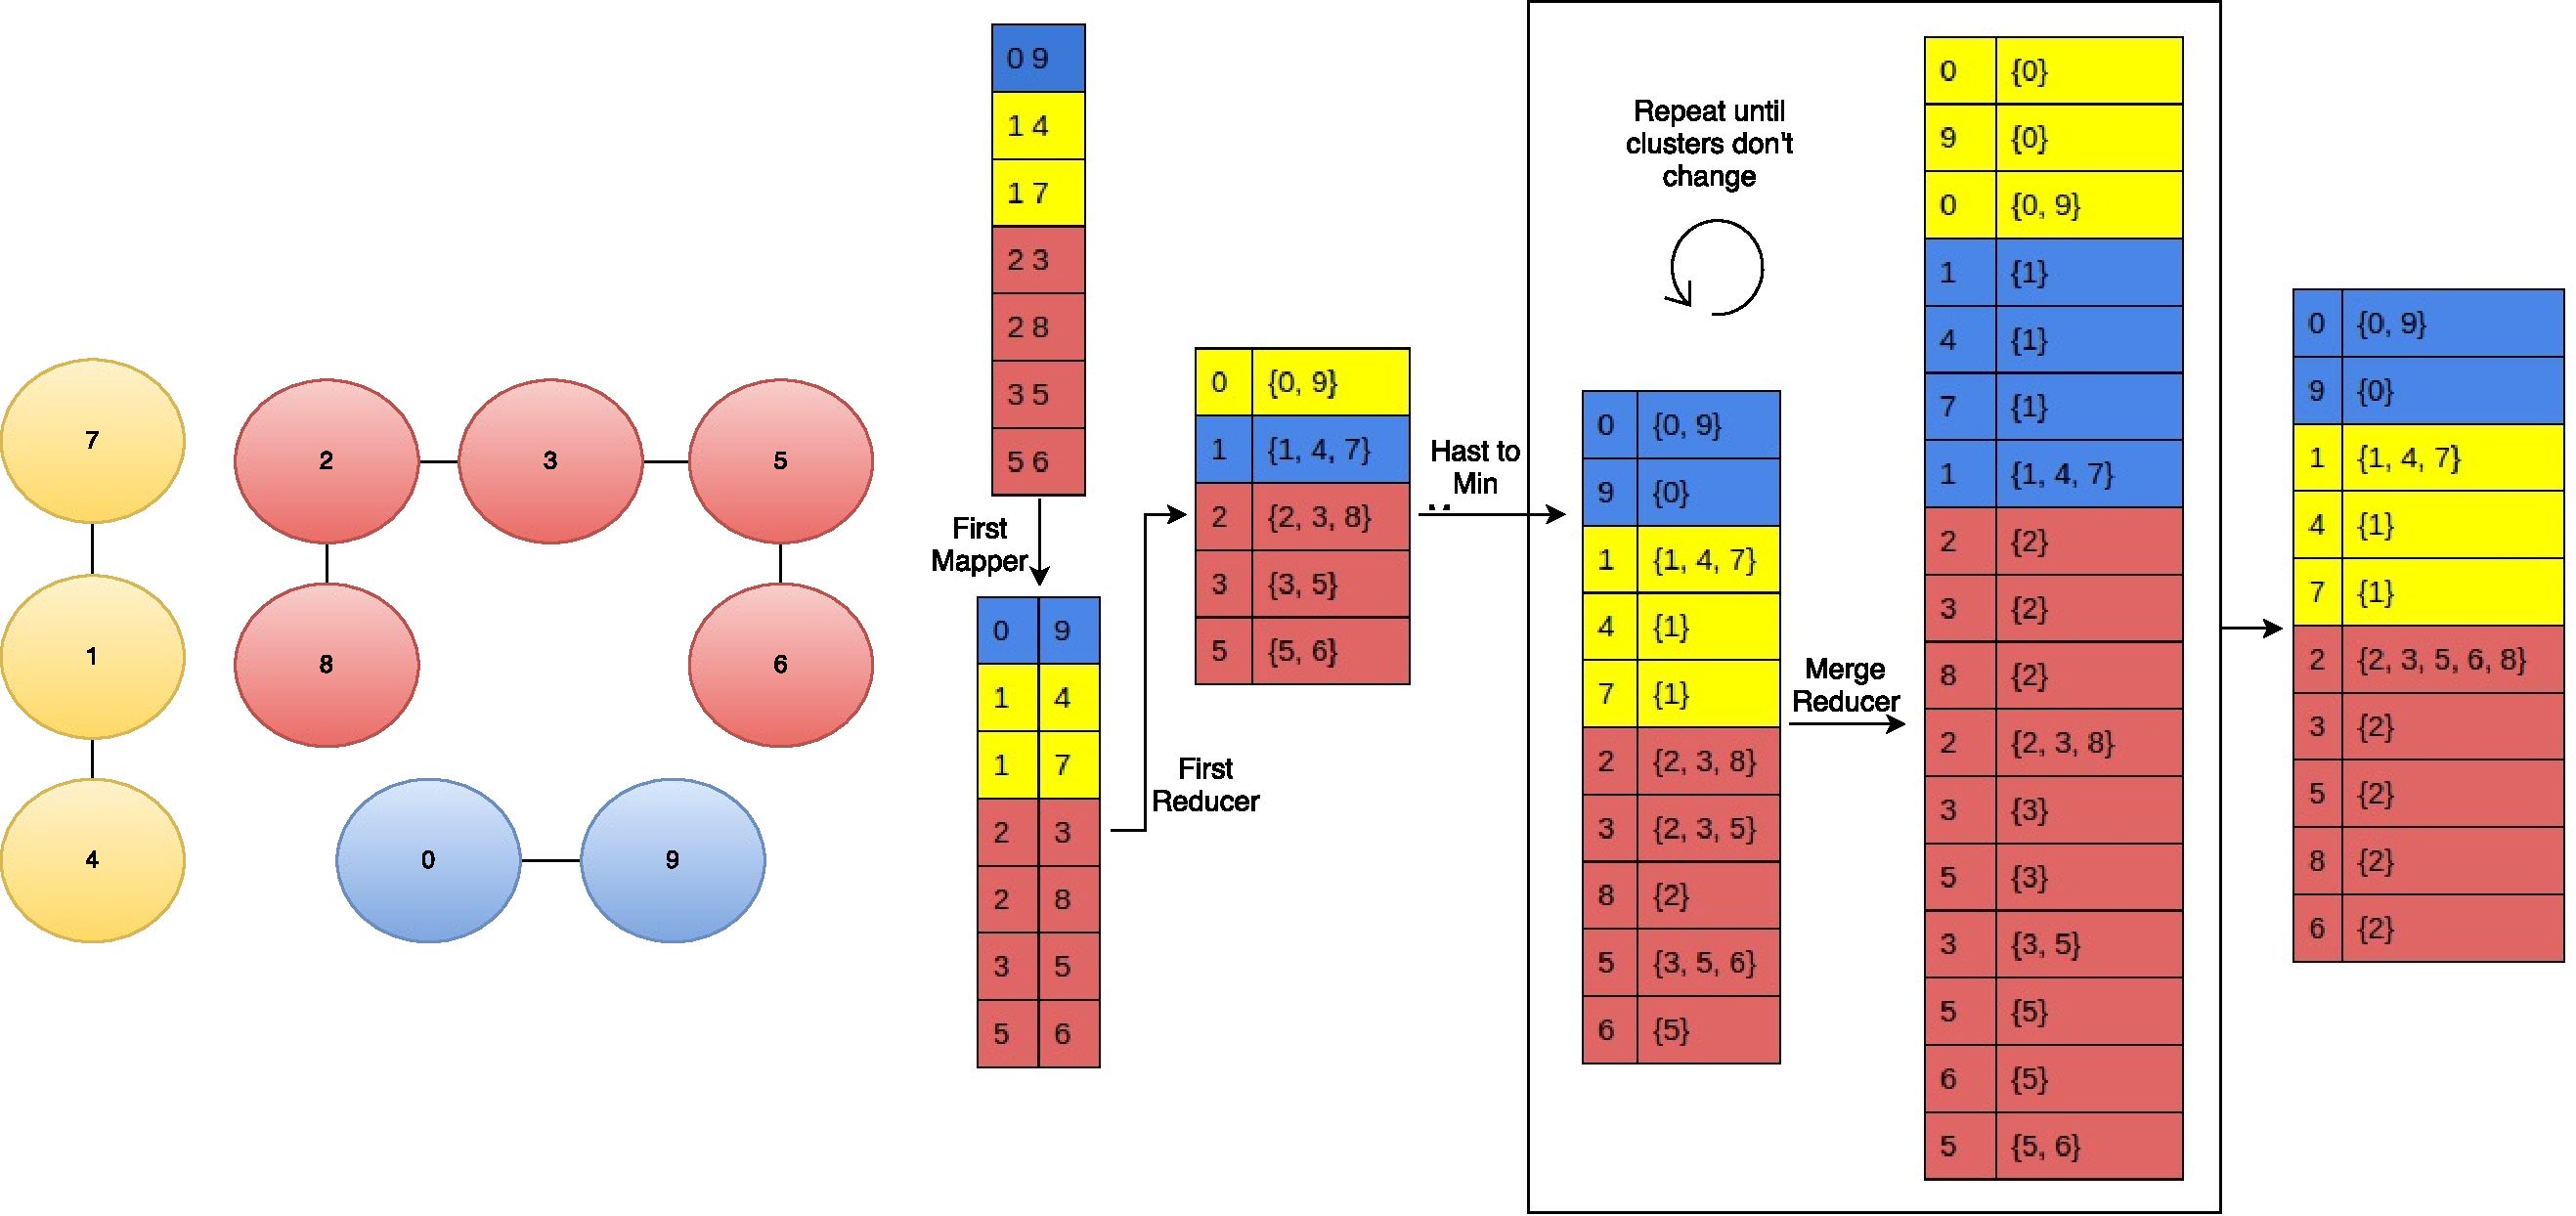
\includegraphics[width=40pc]{figures/mapreduce_example.pdf}
 		\caption{Example run of Hast-to-min algorithm}
 		\label{figure:mapreduce_example}
	\end{minipage}
\end{tabular}
\end{figure*}

The analysis that follows for both the sequential and Map-Reduce parts assumes a graph G that can be formalized as $G=(V,E)$ where $V$ is the set of vertices in the graph labeled from $0 \to N-1$ where $N=|V|$ and $E$ is the edges set, which is a set of of 2-element subsets in $V$, that is $E \subseteq \{\{u,v\}: \in V\}$.

\subsection{Sequential}
A sequential algorithm of calculating connected components is used as a proof of concept to show the differences in performance when using Map-Reduce and compare when to use one approach over the other.

We chose to implement a variation of Tarjan's algorithm to find strongly connected components. Although this algorithm calculates strongly connected components in directed graphs, it can be used to find connected components in undirected graphs as well. Algorithm \ref{algo:tarjan} provides the pseudocode of our implementation. It is based on \cite{tarjan}. Essentially, it follows a Depth-First-Search (DFS) approach in exploring the graph and keeps track of the oldest ancestor it has found to associate as the leader of a connected component.

\begin{algorithm}
	\caption{Connected Components}
	\label{algo:tarjan}
	\begin{algorithmic}[1]
		\State Parse edges file
		\State Initialize graph as an adjacency list
		\State Initialize visited, stack, components
		\For {node $v \in nodes $}
			\If {$v \notin visited $}
				\State dfs($v$)
			\EndIf
		\EndFor
		\Function{dfs}{$v$}
			\State $visited[v] = true$
			\State $stack.push(v)$
			\State $isComponentRoot = true$
			\For {node $u \in neighbors(v)$}
				\If {$v \notin visited $}
					\State dfs($v$)
				\EndIf
				\If {$lowLink[u] > lowLink[v]$}
					\State $lowLink[u] = lowLink[v]$
					\State $isComponentRoot = false$
				\EndIf
			\EndFor
			\If {$isComponentRoot$}
				\State Construct component c from stack
				\State components.add(c)
			\EndIf
		\EndFunction
	\end{algorithmic}
\end{algorithm}

\begin{algorithm}[!h]
	\caption{Initialization Step}
	\label{algo:first_step}
	\begin{algorithmic}[1]
		\Function{Map}{$key, value$}
			\State $edge = value.split() $
			\State $emit(edge[0], edge[1])$
		\EndFunction
		\Function{Reduce}{$key, List<value>$}
			\State $outKey = new StringBuilder()$
			\For {$value \in List<value>$}
				\State $outKey.append(clusterSeparator).append(value)$
			\EndFor
			\State $emit(key, outKey)$
		\EndFunction
	\end{algorithmic}
\end{algorithm}

\begin{algorithm}[!h]
	\caption{Iterative Map-Reduce step}
	\label{algo:second_step}
	\begin{algorithmic}[1]
		\Function{Map}{$key, value$}
			\State $clusterNodes = parse(value)$
			\State $clusterNodes = cluster.split(clusterSeparator)$
			\State $v_{min} = min(node \in clusterNodes)$
			\For {$u \in clusterNodes$}
				\State $emit(u, v_{min})$
			\EndFor
			\State $emit(v_{min}, cluster)$
		\EndFunction
		\Function{Reduce}{$key, List<value>$}
			\State Initialize mergedCluster, maxSize
			\For {$C_v \in List<value>$}
				\State $elementsC_v = C_v.split(clusterSeparator)$
				\If {$elementsC_v.length > maxSize$}
					\State $maxSize = elementsC_v.length$ 
				\EndIf
				\State $mergedCluster.add(elementsC_v)$
			\EndFor
			\State $cluster = mergedCluster.toString()$
			\If {$maxSize < mergedCluster$}
				\State $context.counter++$
			\EndIf
			\State $emit(key, cluster)$
		\EndFunction
	\end{algorithmic}
\end{algorithm}

The algorithm's complexity is linear in the number of edges and nodes in the graph, \ie $O(|V| + |E|)$. This means that the algorithm will be very efficient for relatively small graphs, but it will start being ineffective while the graphs grow bigger and bigger up to hundreds of million vertices and edges. In particular, the parsing time of the input file would be the bottleneck since it has to be done sequentially as well as the available memory on the machine we are using, since the graph has to fit in its memory for Algorithm \ref{algo:tarjan} to work. Map-Reduce helps to eliminate exactly these restrictions, since the parsing can be performed in parallel in addition to running the actual connected components algorithm in a parallel fashion.

\subsection{Map-Reduce}

\subsubsection{Hash-to-min}


One of the algorithms that we chose for the Map-Reduce part is based on the Hash-to-Min algorithm introduced in \cite{rastogi}. This algorithm works in multiple logarithmic Map-Reduce rounds  to calculate the connected components of a graph at the end. In each round the algorithm merges overlapping clusters to compute connected components. Essentially, the algorithm can be imagined as a different Breadth-First-Search (\eg BFS) being performed in parallel. Each BFS builds up a connected component by combining smaller ones until there is convergence and the whole connected component has been discovered.

The are basically two phases in our Hash-to-min program for computing connected components. The first phase is the initialization phase which parses the input file and creates the graph as an adjacency list. The mapper emits a key-value pair for each edge in the graph and the reducer accumulates edges for each node and creates a mapping between nodes and list of neighbors. Algorithm \ref{algo:first_step} provides the pseudocode of this phase which is quite simple to follow.

Here comes the first optimization we performed in the original code using the Map-Reduce platform. The input file is processed in parallel using multiple mappers, thus utilizing the parallelism that we inherently get by running our program on Map-Reduce. For huge graphs, this phase should take less to complete than running on a single machine. It also overcomes any memory issues for storing the complete graph in memory on a single machine, since the graph is created in a distributed fashion by the reducers.

The second phase of Map-Reduce is the iterative step which merges together smaller connected components to form large ones in each iteration until convergence is achieved (\ie until there are no changes in the connected components calculated). Algorithm \ref{algo:second_step} shows the approach we follow in this Map-Reduce job. The map function calculates the minimum node in each cluster which we call $v_min$. Then it emits $(u, v_min)$ for each node $u$ in the cluster and also $(v_min, cluster)$. This aggregates the connected component to $v_min$ while reassuring that the rest of the nodes are associated with $v_min$ to avoid creating duplicate connected components. This is the second optimization in our approach. The alternative here would be to emit the cluster to each node, but that would only bloat the number of data being transmitted and add an additional overhead. Only one node is enough to represent the whole connected component and therefore an easy choice is to use the minimum labeled node as the component's representative. The reducer then takes all the clusters that are associated with one node and merges them together. If the final cluster has changed, we increment a counter to indicate this. If no more changes have taken place, the algorithm has converged. As shown in \cite{rastogi}, the algorithm will converge in $O(logn)$ steps, where $n$ is the total number of nodes in the graph.

The algorithm's complexity is linear in the number of edges and nodes in the graph, \ie $O(|V| + |E|)$. This means that the algorithm will be very efficient for relatively small graphs, but it will start being ineffective while the graphs grow bigger and bigger up to hundreds of million vertices and edges. In particular, the parsing time of the input file would be the bottleneck since it has to be done sequentially as well as the available memory on the machine we are using, since the graph has to fit in its memory for Algorithm \ref{algo:tarjan} to work. Map-Reduce helps to eliminate exactly these restrictions, since the parsing can be performed in parallel in addition to running the actual connected components algorithm in a parallel fashion.

\subsubsection{Two-Phase}

The other one we picked is based on the Two-Phase algorithm presented in \cite{kiveris}. It first introduces two operations over a graph and then how to combine them in order to to find the connected components.

Let $G = (V,E)$ and undirected graph, on $n = |V|$ nodes, and $m = |E|$ edges. For a node $v$, we denote by $\Gamma(v) = \{w|(v,w) \in E\}$ the neighbors of $v$ and $\Gamma^{+}(v) = \Gamma(v) \cup \{v\}$ as neighborhood of v and itself. Also, every node $v$ in the graph is associated with a real number label $l_{v}$. We now show the operations, which preserves the connectivity of the graph when performing them at all nodes in parallel.

\begin{algorithm}[!h]
        \caption{Small-star operation}
        \label{algo:small_star}
        \begin{algorithmic}[1]
                \Function{Map}{$u, v$}
                        \If {$l_{u} \leq l_{v}$}
                                \State $emit(u, v)$  
                        \Else
                                \State $emit(v, u)$  
                        \EndIf
                \EndFunction
                \Function{Reduce}{$u, N \subseteq \Gamma(u)$}
                        \State $m = u$
                        \For {$v \in N$}
                                \If {$l_v < l_m$}
                                        \State $m = v$
                                \EndIf
			\EndFor
                        \For {$v \in N$}
                                \State $emit(v, m)$
                        \EndFor
                \EndFunction
        \end{algorithmic}
\end{algorithm}


\begin{algorithm}[!h]
        \caption{Large-star operation}
        \label{algo:large_star}
        \begin{algorithmic}[1]
                \Function{Map}{$u, v$}
                        \State $emit(u, v)$
                        \State $emit(v, u)$
                \EndFunction
                \Function{Reduce}{$u, \Gamma(u)^{+}$}
                        \State $m = u$
                        \For {$v \in N$}
                                \If {$l_v < l_m$}
                                        \State $m = v$
                                \EndIf
                        \EndFor
                        \For {$v \in N$}
                                \If {$l_v > l_u$}
                                        \State $emit(v, m)$
                                \EndIf
                        \EndFor
                \EndFunction
        \end{algorithmic}
\end{algorithm}

\begin{figure}[ht]
  \centering
    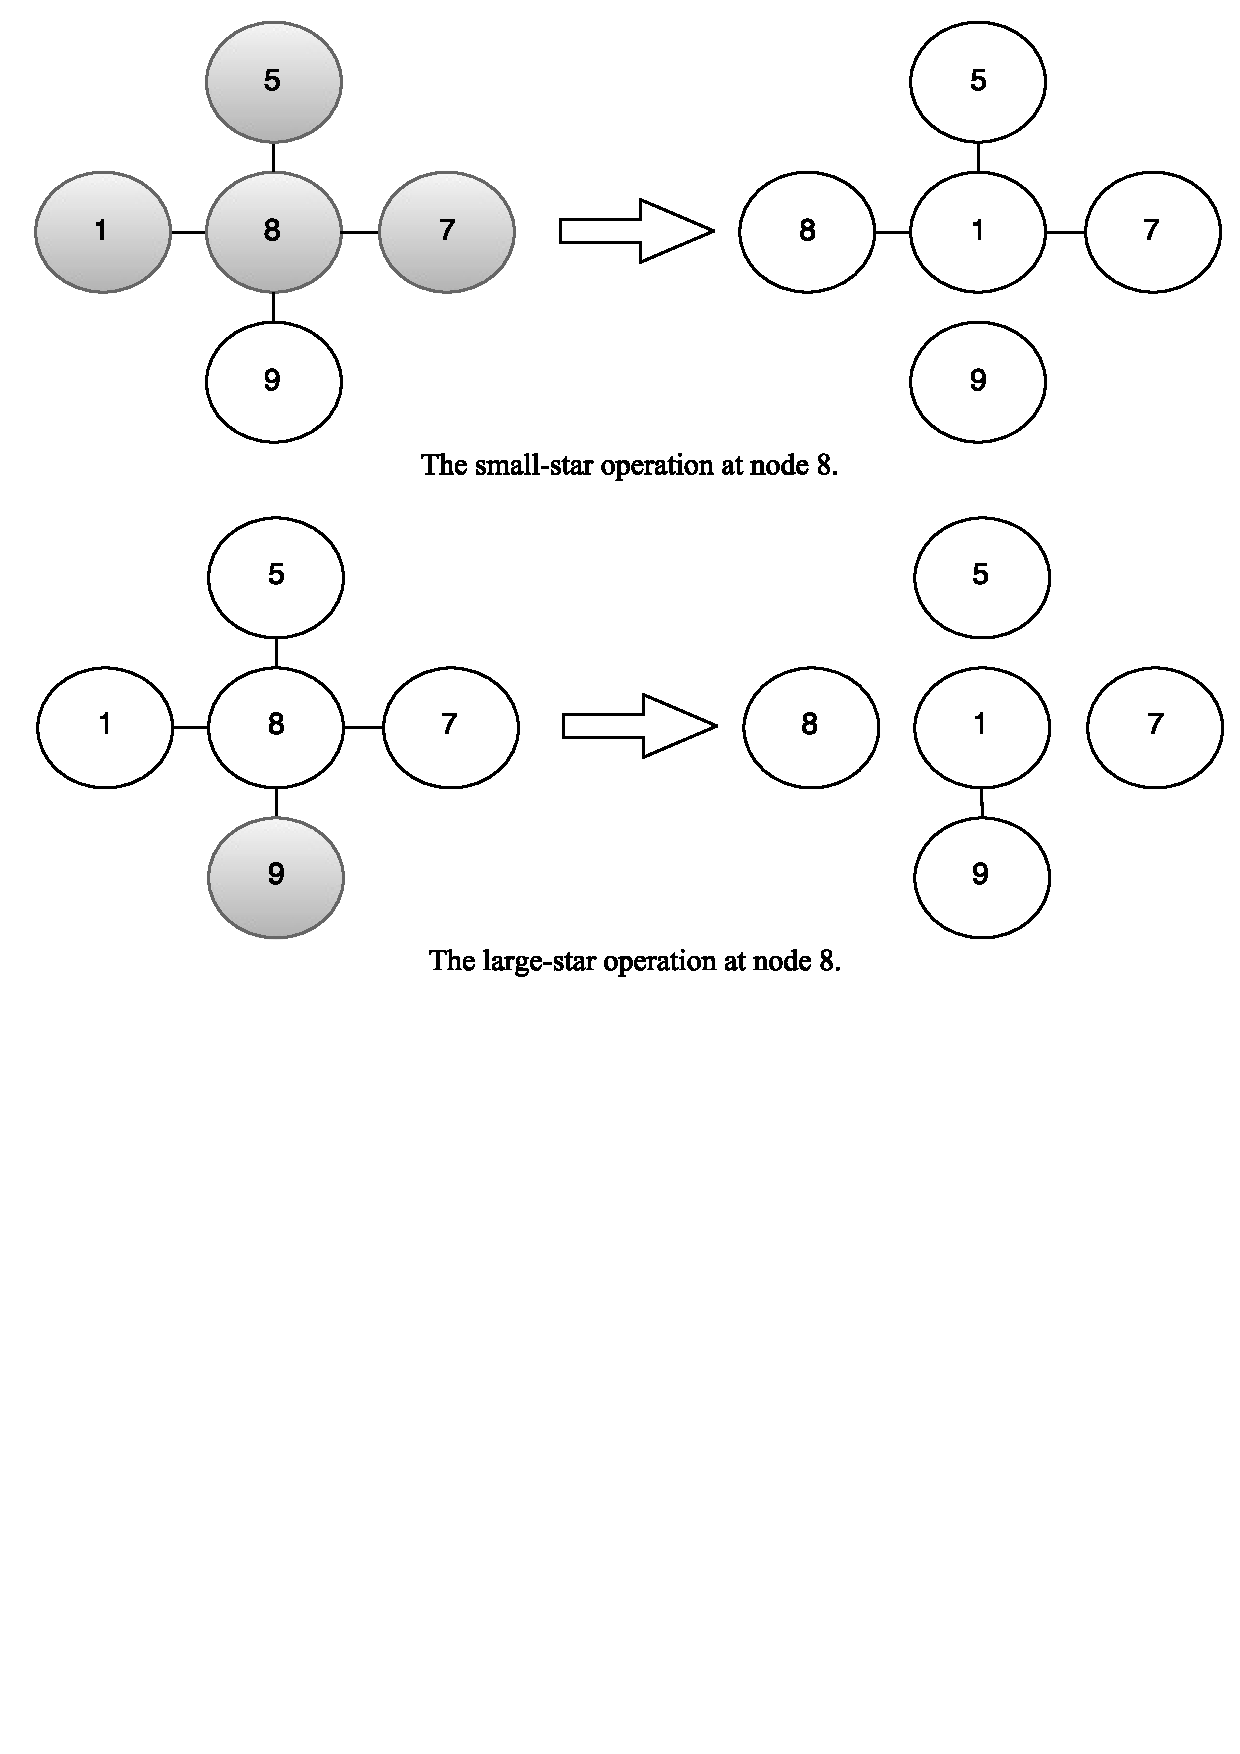
\includegraphics[width=20pc]{figures/two_phase}
  \caption{Small and large star operations}
  \label{fig:smalllargestar}
\end{figure}

This two operations can be combined and create the two phase algorithm. In each phase, large-star is repeated until convergence followed by one small-star operation.

\begin{algorithm}[!h]
        \caption{Two-Phase Algorithm}
        \label{algo:two_phase}
        \begin{algorithmic}[1]
                \Function{Two Phace}{}
                        \Repeat
                                \Repeat
                                        \State $large-star$
                                \Until{Convergence}
                        \State $small-star$
                        \Until{Convergence}
                \EndFunction
        \end{algorithmic}
\end{algorithm}

iThe Two-Phase Algorithm converges after $O(log^2 n)$ Map-Reduce rounds, which is higher than the Hash-to-min. The advantage it provide is a smaller communication size, making it able to handle bigger graphs in theory.

Intuitively this algorithm efficiently simulates the classical Union-Find algorithm in parallel. In the inner-loop each node, finds its local-minimum and adds an edge to it (this is equivalent to path compression). In the outer loop, distinct local minimums are connected and then joined in a union step. \cite{kiveris}

\section{Experiments}\label{sec:exp}
\subsection{Datasets}

All the input files we used consist of edges making it straightforward to parse them as showed in \ref{fig:graphfileformat}.

\begin{verbbox}
node_from_1 node_to_1
node_from_2 node_to_2
...
node_from_n node_to_n
\end{verbbox}

\begin{figure}[ht]
  \centering
  \theverbbox
  \caption{Graph file format}
  \label{fig:graphfileformat}
\end{figure}

We used different graph files taken from \cite{datasets} to measure both the Sequential and Map-Redude algorithm performance. The following table describes different metrics of each one:

\begin{table}[h!]
\footnotesize
\begin{center}
\begin{tabular}{|c|c|c|c|}
\hline
{\bf Name} & {\bf Nodes}& {\bf Edges} & {\bf Size}\\
\hline
\hline
simple\_graph   & 10  & 14  & 55 bytes  \\
\hline
medium\_graph   & 534  & 9626  & 96.2 Kb  \\
\hline
ego-Facebook   & 4039  & 88234  & 854.4 Kb  \\
\hline
ego-Gplus   & 107614  & 13673453  & 1.2GB  \\
\hline
big\_graph   & -  & -  & 2.4GB  \\
\hline
\end{tabular}
\caption{Graphs}
\label{tb:graphfiles}
\end{center}
\end{table}

\subsection{Sequential}
We used an implementation of Tarjan's Algorithm that has $O(|V| + |E|)$ worst case performance. It uses a Depth-First-Approach (DFS) as described in Section \ref{sec:algo}. It begins at an arbitrary node and  visits every node of the graph exactly once. As it is going through the graph it will be generating the various connected components.

\begin{table}[!h]
\footnotesize
\begin{center}
\begin{tabular}{|c|c|c|}
\hline
{\bf Graph} & {\bf Time (milliseconds)}& {\bf components \#} \\
\hline
\hline
simple\_graph   & 0  & 3  \\
\hline
medium\_graph   & 4  & 2   \\
\hline
ego-Facebook   & 11  & 1325  \\
\hline
ego-Gplus   & 812 & 37249 \\
\hline
big\_graph   & -  & -  \\
\hline
\end{tabular}
\caption{Sequential times}
\label{tb:sequentialtimes}
\end{center}
\end{table}

The results here are as expected. The algorithm performs really well when using small files and the total execution time is really small. However, we can see that as the files grow bigger and bigger the parsing time starts becoming the dominating factor that takes up more than half of the total execution time.

\subsection{Map-Reduce}

Table \ref{tb:MapReducetimes} contains the execution time for the Map-Reduce implementation for each input graph file. We can see that using Map-Reduce for really small files is not very efficient but the real advantage is when using it to process large files. Specifically,  using Map-Reduce we were able to process the big\_graph file which failed on a single machine due to memory limitations.

\begin{table}[h!]
\footnotesize
\begin{center}
\begin{tabular}{|c|c|c|}
\hline
{\bf Graph} & {\bf Phase 1 (sec)} & {\bf Phase 2 (sec)}\\
\hline
\hline
simple\_graph   & 23  & 82 \\
\hline
medium\_graph   & 12 & 60 \\
\hline
ego-Facebook   & 30 & 150 \\
\hline
ego-Gplus   & 60  & 220 \\
\hline
big\_graph   & 240 & 1740 \\
\hline
\end{tabular}
\caption{Map-Reduce times}
\label{tb:MapReducetimes}
\end{center}
\end{table}



\section{Conclusion}\label{sec:conclusion}
Opting over a distributed approach in finding connected components in a graph, is evidently faster for ever-increasing size of graphs. The algorithm fails to work sequentially on a large graph (estimated to have 200,000 nodes). The very same graph gets computed in only 33 minutes using \textit{Hadoop MapReduce} via \textit{AmazonWebServices}.

With this we can conclude that for very large graphs, using map reduce paradigm gives a time-complexity of \textit{$O(logn)$} steps by parallel runs as compared to the traditional linear complexity of \textit{$O(|V| + |E|)$}, but if the input graph data-set is small then the sequential algorithm can save us from the overhead  (\eg Initialization of tasks/jobs, communication between mappers and reducers, generation of intermediate outputs, etc.) of map-reduce paradigm.


% A category with the (minimum) three required fields
%\category{H.4}{Information Systems Applications}{Miscellaneous}
%A category including the fourth, optional field follows...
%\category{D.2.8}{Software Engineering}{Metrics}[complexity measures, performance measures]

%\terms{Theory}

%\keywords{ACM proceedings, \LaTeX, text tagging} % NOT required for Proceedings


%
% The following two commands are all you need in the
% initial runs of your .tex file to
% produce the bibliography for the citations in your paper.
\bibliographystyle{abbrv}
\bibliography{bibliography}  % sigproc.bib is the name of the Bibliography in this case
% You must have a proper ".bib" file
%  and remember to run:
% latex bibtex latex latex
% to resolve all references
%
% ACM needs 'a single self-contained file'!
%
%APPENDICES are optional
%\balancecolumns
%\appendix
%Appendix A

%\subsection{References}

\balancecolumns
% That's all folks!
\end{document}
